\section{Recursive Environment Evolution}
\label{sec:evolution}

MAW expands the task distribution within existing executable environments. It composes reference task graphs, reconstructs coherent user requests, and accepts tasks only after strict execution and quality checks. 

\subsection{Recursive Task Composition}
\label{sec:composition}

\paragraph{Seed tasks and task graphs.}
Our seed construction follows the executable-tool and graph-guided synthesis approach illustrated by ToolVerse~\citep{zhou2026toolverse}: real MCP tool schemas guide the construction of mock databases and executable tool functions, tool-graph sampling proposes call sequences, and execution provides evidence for reverse task synthesis. Each seed supplies a functional goal and a reference task DAG $H=(N,A)$, whose nodes represent tool-call instances and whose edges represent data or state dependencies. Composition operates on tasks from a compatible environment.

Let $\mathcal C_0$ be the seed pool. At round $r$, $\operatorname{Compose}_z$ combines compatible candidates in $\mathcal C_r$, where $z\in\{\mathrm{serial},\mathrm{parallel}\}$. Retained candidates can be used in later rounds, allowing a composite task to acquire further goals and dependencies. The provenance record preserves its parent tasks for tracing the construction.

\paragraph{Serial composition.}
Serial composition connects goals through an output or state effect required by a downstream operation. A first subtask may identify the records that a second subtask must inspect, or create an object that it subsequently modifies. The proposed edge must correspond to a usable dependency in the reconstructed execution. An arbitrary ordering between independent calls does not provide this dependency.

\paragraph{Parallel composition.}
Parallel composition combines goals that can progress independently before their results are integrated into a joint report, comparison, or decision. Compatible reads may be shared during reconstruction, but shared work is not a third composition operator. Calls are merged only when their arguments and state assumptions support the same use; matching tool names alone is insufficient.

Applying these two operators recursively produces candidates with mixed serial and parallel structure. The candidate DAG guides reconstruction; its size does not determine the number of calls required by the final task. Figure~\ref{fig:task-statistics} therefore compares seed references with reconstructed, accepted references. The audited snapshot uses two-parent candidates; its statistics do not measure gains from multiple recursive rounds (Appendix~\ref{app:synthesis}).

\begin{figure}[t]
  \centering
  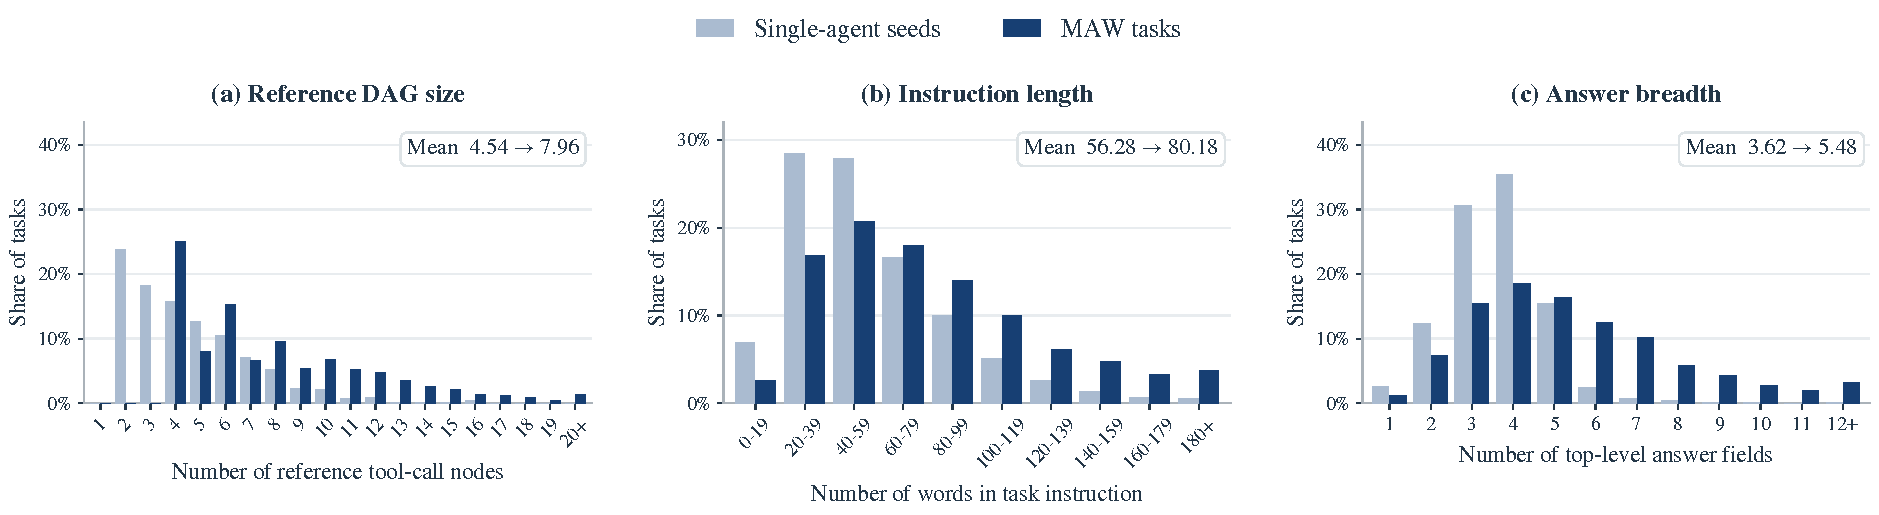
\includegraphics[width=\linewidth]{figures/task_statistics.pdf}
  \caption{\textbf{Seed and accepted-task statistics.}
Distributions of reference tool-call counts, instruction lengths (in words), and top-level answer-field counts for 10,860 seeds and 2,581 accepted MAW tasks.
Bars show the fraction of tasks within each cohort; inset labels report means (seeds $\rightarrow$ MAW).
For accepted tasks, reference tool-call counts are measured from the original reference DAGs before plan reconstruction.
Each cohort is normalized separately, and the final bin includes the full tail.
Answer-field counts exclude three seeds with non-dictionary answers.
These statistics describe the audited snapshot and do not measure solver difficulty or training benefit.}
  \label{fig:task-statistics}
\end{figure}

\subsection{Semantic Reconstruction}
\label{sec:reconstruction}

Graph composition specifies how reference operations may be connected, but does not yet provide a coherent user request. Parent tasks can refer to different entities, time ranges, or reporting requirements. Semantic reconstruction uses the candidate DAG, parent goals, and executable tool context to formulate a single request, instantiate tool arguments, and construct a reference plan. It may align entities, remove redundant calls, or add a lookup needed to support the combined goal. The request states the desired outcome without exposing the reference plan or prescribing worker allocation.

The reconstructed plan is executed to derive the reference answer and required database effects. Where an explicit task DAG is available, its tool nodes, dependency edges, and answer node are checked against that plan and its observed execution. Reconstruction thus connects the proposed graph structure to an executable problem; all final structural statistics must refer to the reconstructed artifact.

\begin{figure}[t]
  \centering
  
\includegraphics[width=\linewidth]{figure3.pdf}
  \caption{\textbf{DAG composition and semantic reconstruction.} Parent goals and reference operations provide the input. Serial or parallel composition proposes a candidate graph; reconstruction aligns its context into a coherent request and may revise the reference calls. Execution checks the resulting reference. The example illustrates the mechanism.}
  \label{fig:composition-example}
\end{figure}

\subsection{Execution and Quality Gates}
\label{sec:validation}

Repeated composition can accumulate redundant calls or combine incompatible requirements. MAW uses two levels of validation to keep these defects out of the accepted training set. \emph{Execution validation} first runs the reconstructed reference in an isolated, reset environment. It checks tool and argument validity, computes the answer from actual observations, and records final database changes. The generated solution is then replayed from the same initial conditions; its answer and final state must pass the checker.

\emph{Quality gates} assess whether this executable reference solves a coherent problem. They check fulfillment of the request, answer completeness, preservation of parent goals, workflow coherence, state consistency, and whether repeated operations serve a justified purpose. The audited pipeline requires two separate semantic reviews, each based on the request and execution evidence without seeing the other review's verdict. Both must pass every required check. A failed, uncertain, or missing review prevents acceptance. This screening adds semantic checks to successful execution, while retaining the possibility of shared errors by the review model.

An accepted task packages the request with its resettable environment, answer/state checker, and hidden reference evidence. These artifacts support both rollouts and process scoring. Construction provenance and exact acceptance records are retained separately from policy-visible inputs. Appendix~\ref{app:synthesis} documents the snapshot and its validation coverage.

% \begin{algorithm}[t]
% \caption{Recursive task construction and acceptance}
% \label{alg:synthesis}
% \begin{algorithmic}[1]
% \REQUIRE Seed pool $\mathcal C_0$, executable environments, composition budget $B$
% \STATE $\mathcal C\gets\mathcal C_0$; $\mathcal D\gets\varnothing$
% \WHILE{composition budget remains}
%   \STATE Select compatible parents and $z\in\{\mathrm{serial},\mathrm{parallel}\}$
%   \STATE Compose a candidate DAG and record its parent tasks
%   \STATE Reconstruct a coherent request and executable reference
%   \STATE Execute and replay the reference; verify the answer and final state
%   \IF{execution checks and all required quality gates pass}
%     \STATE Add the task package to $\mathcal D$; retain the candidate for later composition
%   \ENDIF
% \ENDWHILE
% \RETURN $\mathcal D$ and construction/acceptance records
% \end{algorithmic}
% \end{algorithm}

% Algorithm~\ref{alg:synthesis} describes the recursive construction path. The separately audited snapshot freezes its two-parent candidates before reconstruction; the distinction is recorded in Appendix~\ref{app:synthesis}.
